\documentclass[12pt,letterpaper,final]{article}
\usepackage[utf8]{inputenc}
\usepackage{amsmath}
\usepackage{amsfonts}
\usepackage{graphicx}
\graphicspath{ {img/} }
\usepackage{amssymb}
\usepackage{xcolor}
\title{Models for Falling Bodies With Air Resistance}
\date{9/11/2015}
\author{Shawn Hartley}
\begin{document}
\maketitle
\section{Intuition}
Consider an object of mass $m$ that has an initial velocity $v_{0}$ towards the surface of the Earth. In classical mechanics air resistance is ignored and the standard model is 

\[v = g \cdot t + v_{0}\]\\

Ignoring air resistance now days is generally not a very good model. Hundreds of years ago people could choose to ignore it because they could not fly. Most experiments to test falling objects were from the tops of buildings that were several stories tall. The effect of air resistance could be ignored because objects were not dropped from a height where terminal velocity could be reached. There are several ways to think of what air resistance and terminal velocity are. In essence, terminal velocity is reached when a force in equal magnitude counteracts the force of gravity. At that point the object is no longer accelerating and a constant velocity, the terminal velocity, has been reached.\\

\centerline{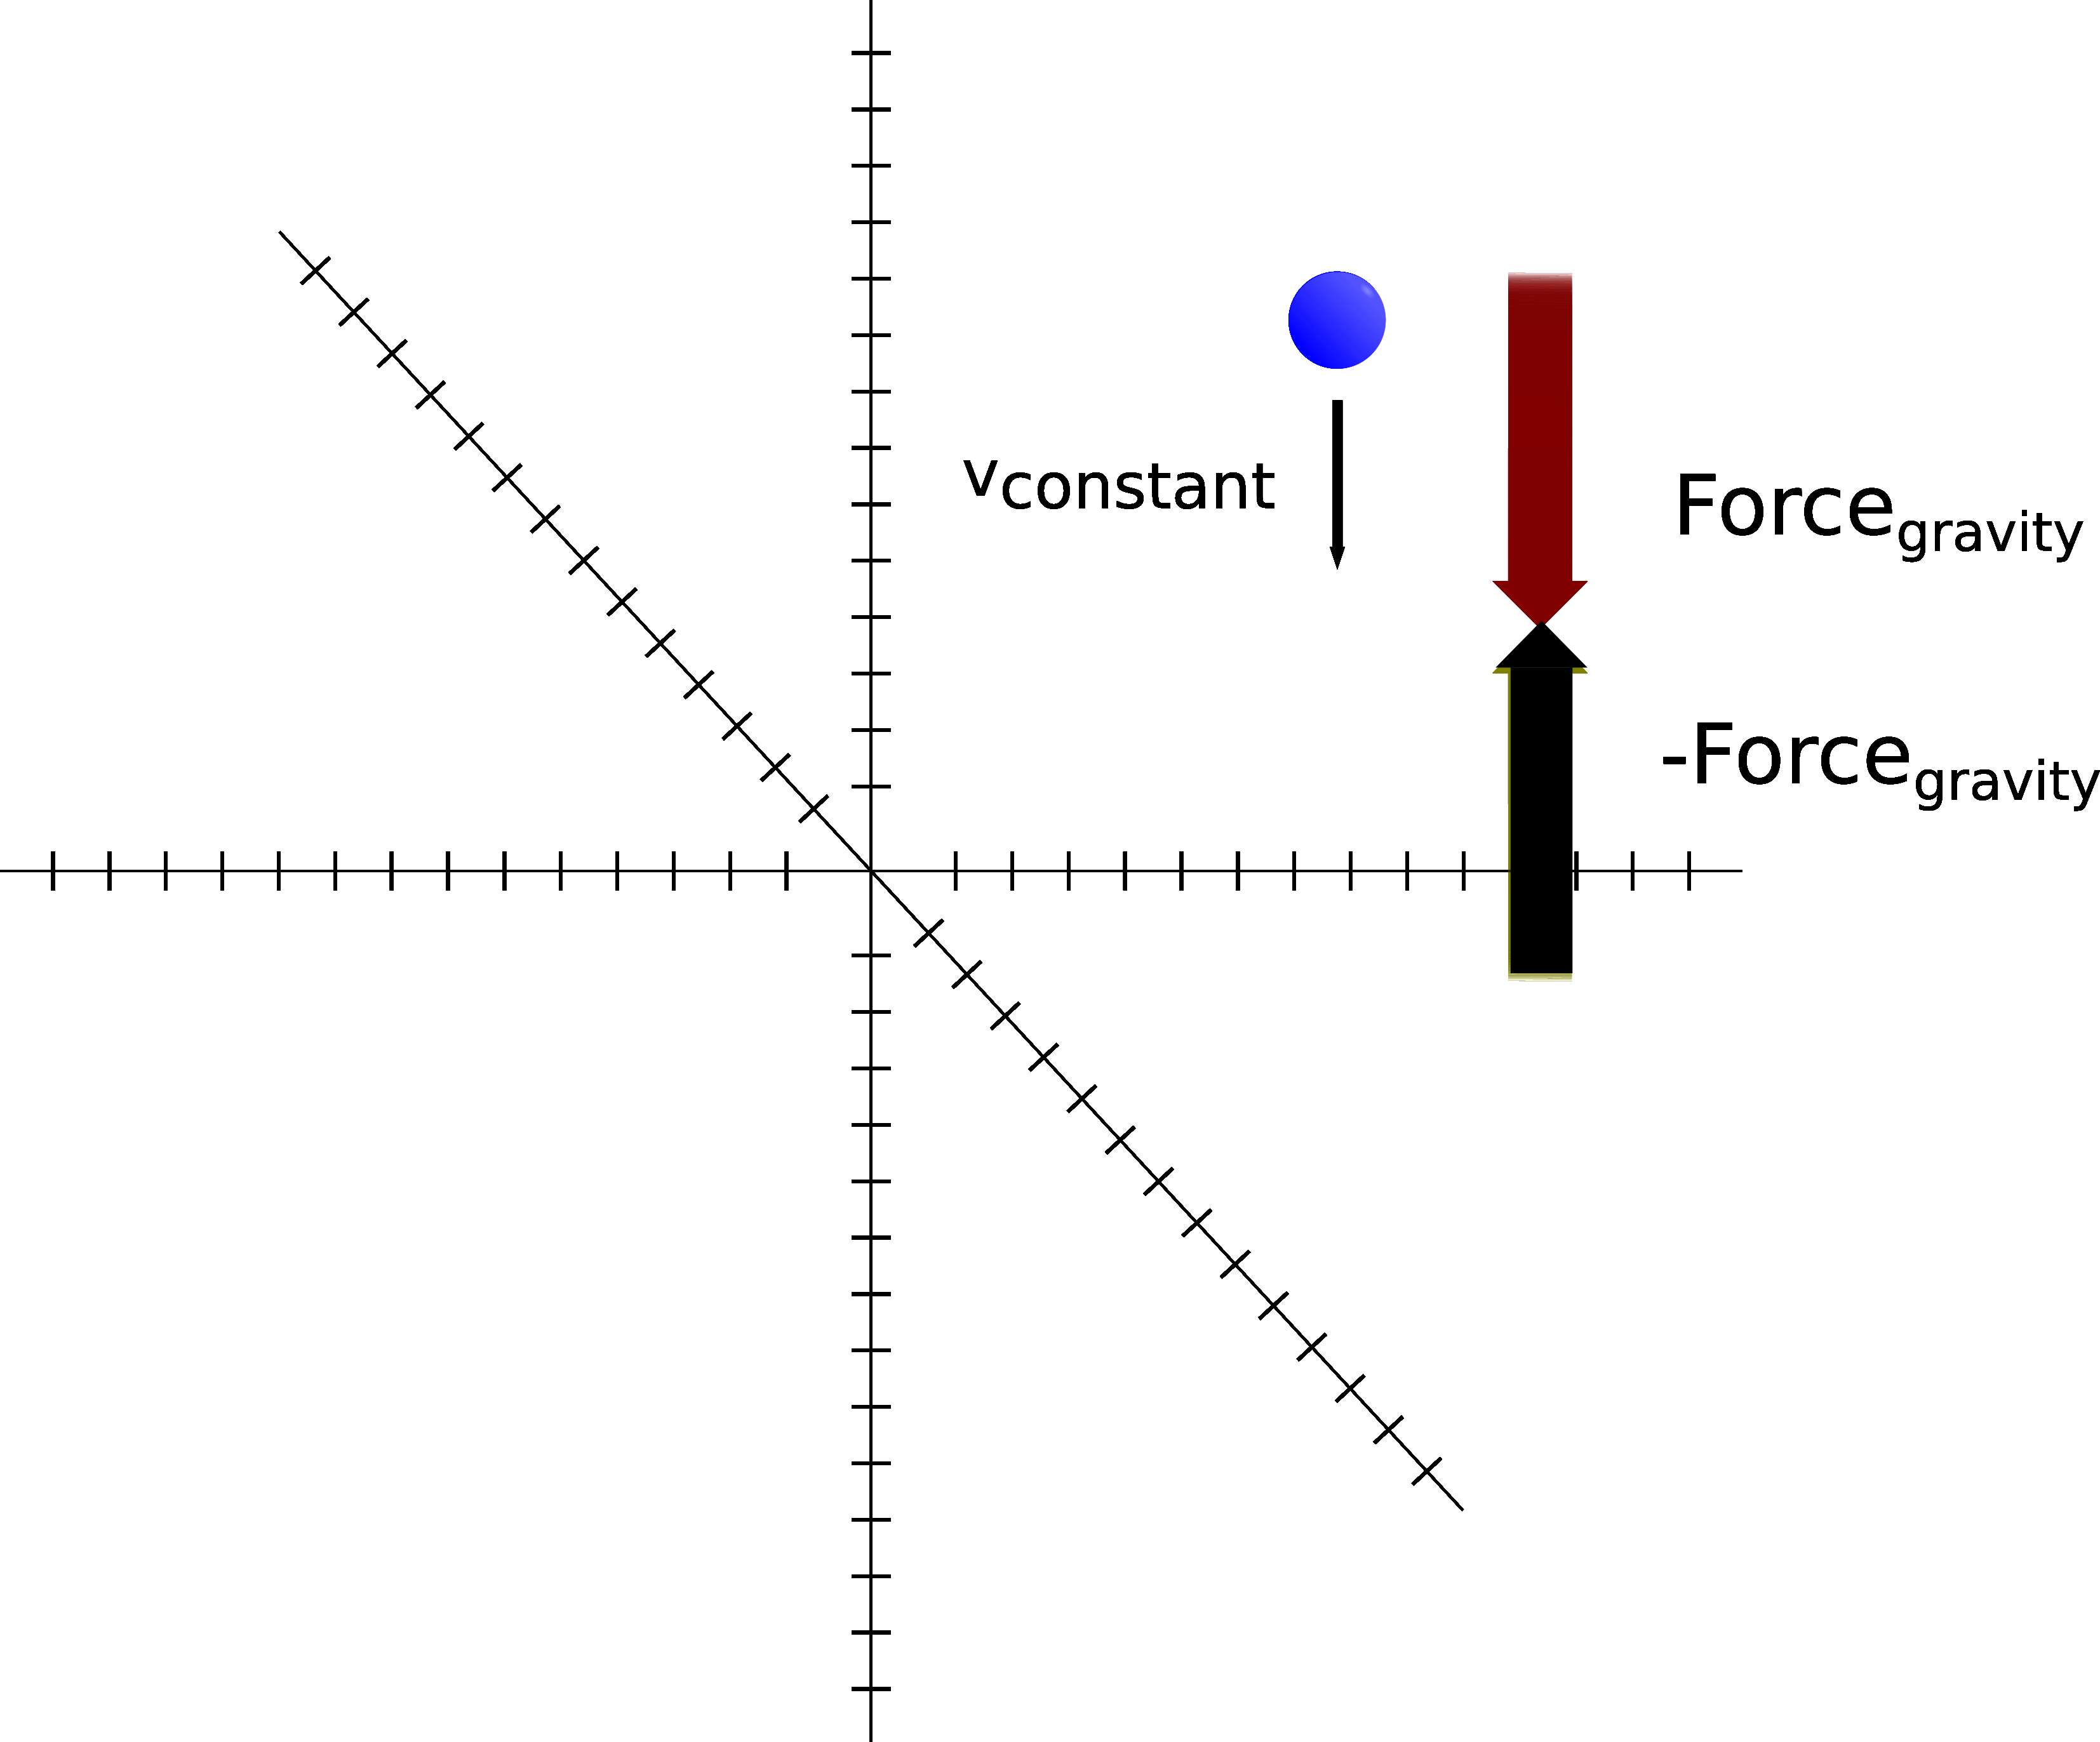
\includegraphics[scale=1]{resistive_force}}
d\centerline{\caption{Figure 1: A force counters the downward force of gravity.}}\\
\\
If an object reaches terminal velocity then the forces must be in equilibrium as can be seen by figure 1. It is known that the force due to gravity is $m \cdot g$. The other force comes from the resistance of an object, of sufficient hardness, pushing through some other mass $\kappa$. Assuming the object is of sufficient hardness, $ie$ it will not break pushing through $\kappa$ , then the question comes to what amount of resistance $\kappa$ offers as the other object collides through it.

\section{Models}
Assuming that the particles of $\kappa$ are stationary relative to the ground then three simple models are easy to construct. The first two will assume\\
\centerline{$F_{\text{Resistance of }\kappa} \propto v^{n}$}\\

Which basically says that $\kappa$'s resistance is proportional to the velocity of some power. In other words as our object collides with $\kappa$ there is an equilibrium between our falling mass's energy with the collision of $\kappa$. These seem like a reasonable place to start, after all anyone who has put their hand out a window going $30\tfrac{km}{hr}$ knows that is less force than putting their hand out the window at $120\tfrac{km}{hr}$.\\

\centerline{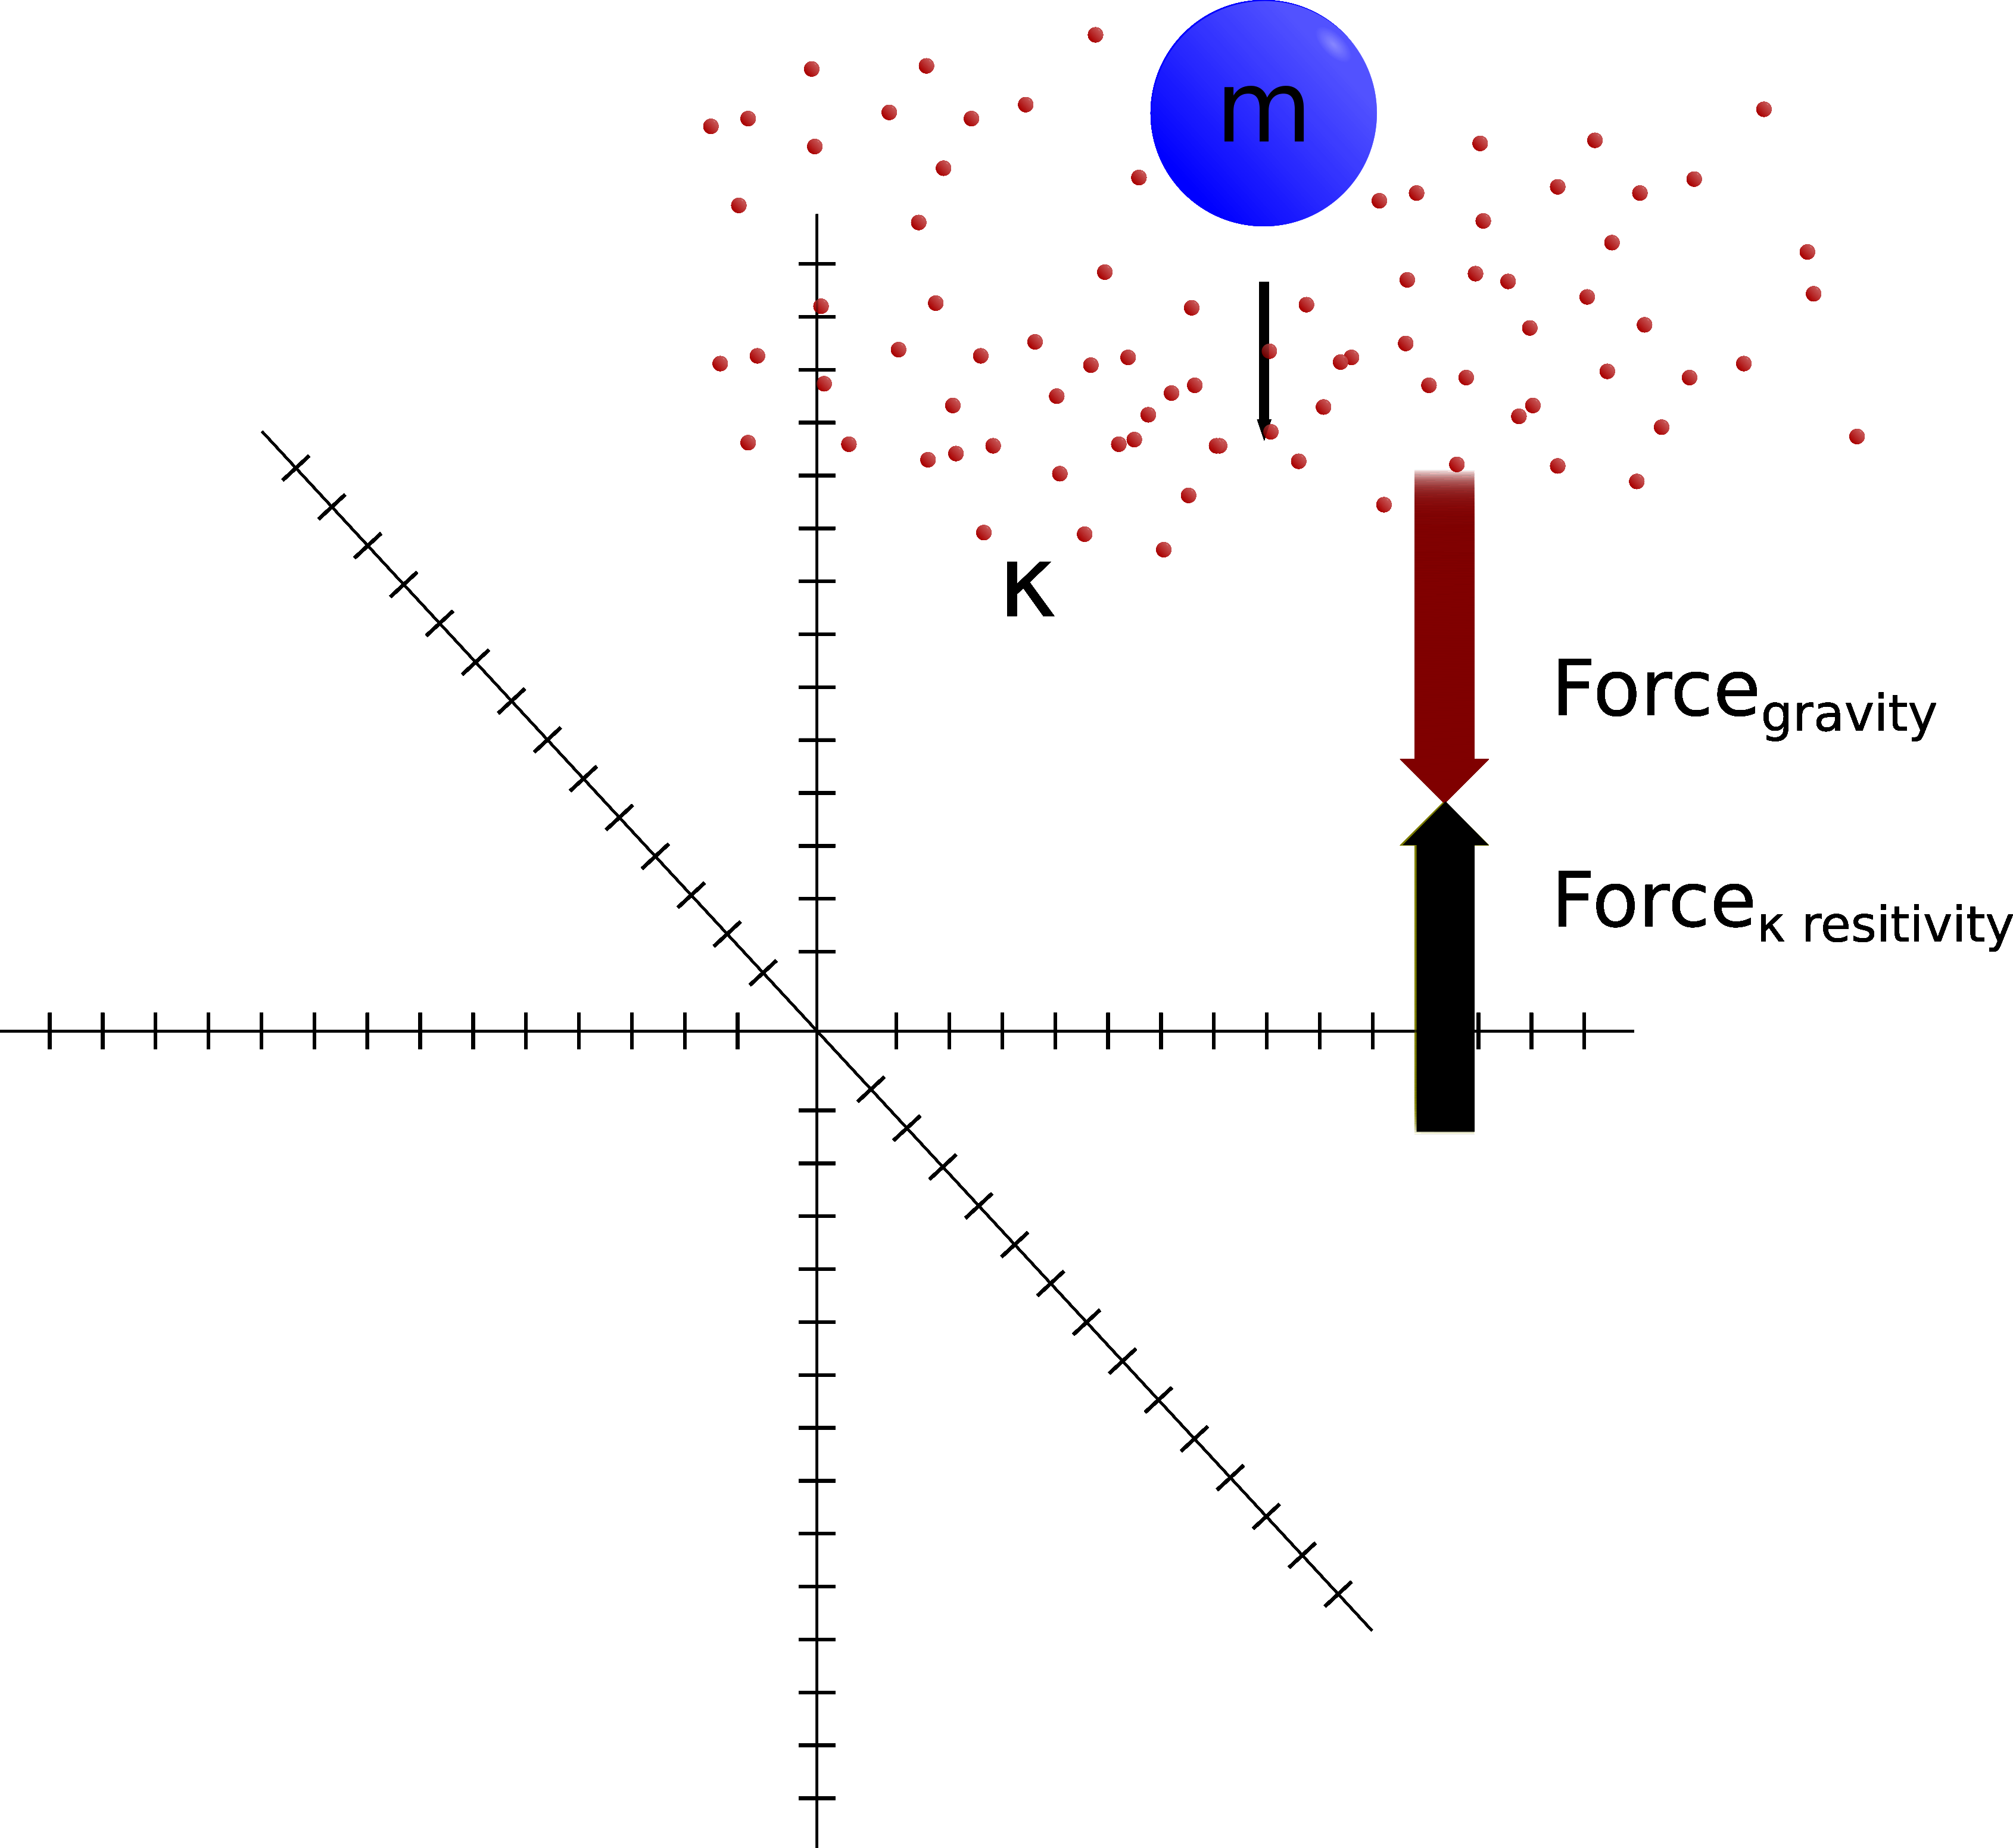
\includegraphics[scale=1]{kappa}}
\centerline{\caption{Figure 2: The force of gravity is at equilibrium with force resulting from the collision with $\kappa$.}}\\
\\
The coordinate system for the models will be defined in the frame of reference of the falling mass. The coordinates will be centered at an initial position and it will move in the positive x direction under the influence of gravity until a terminal velocity is reached.\\

\centerline{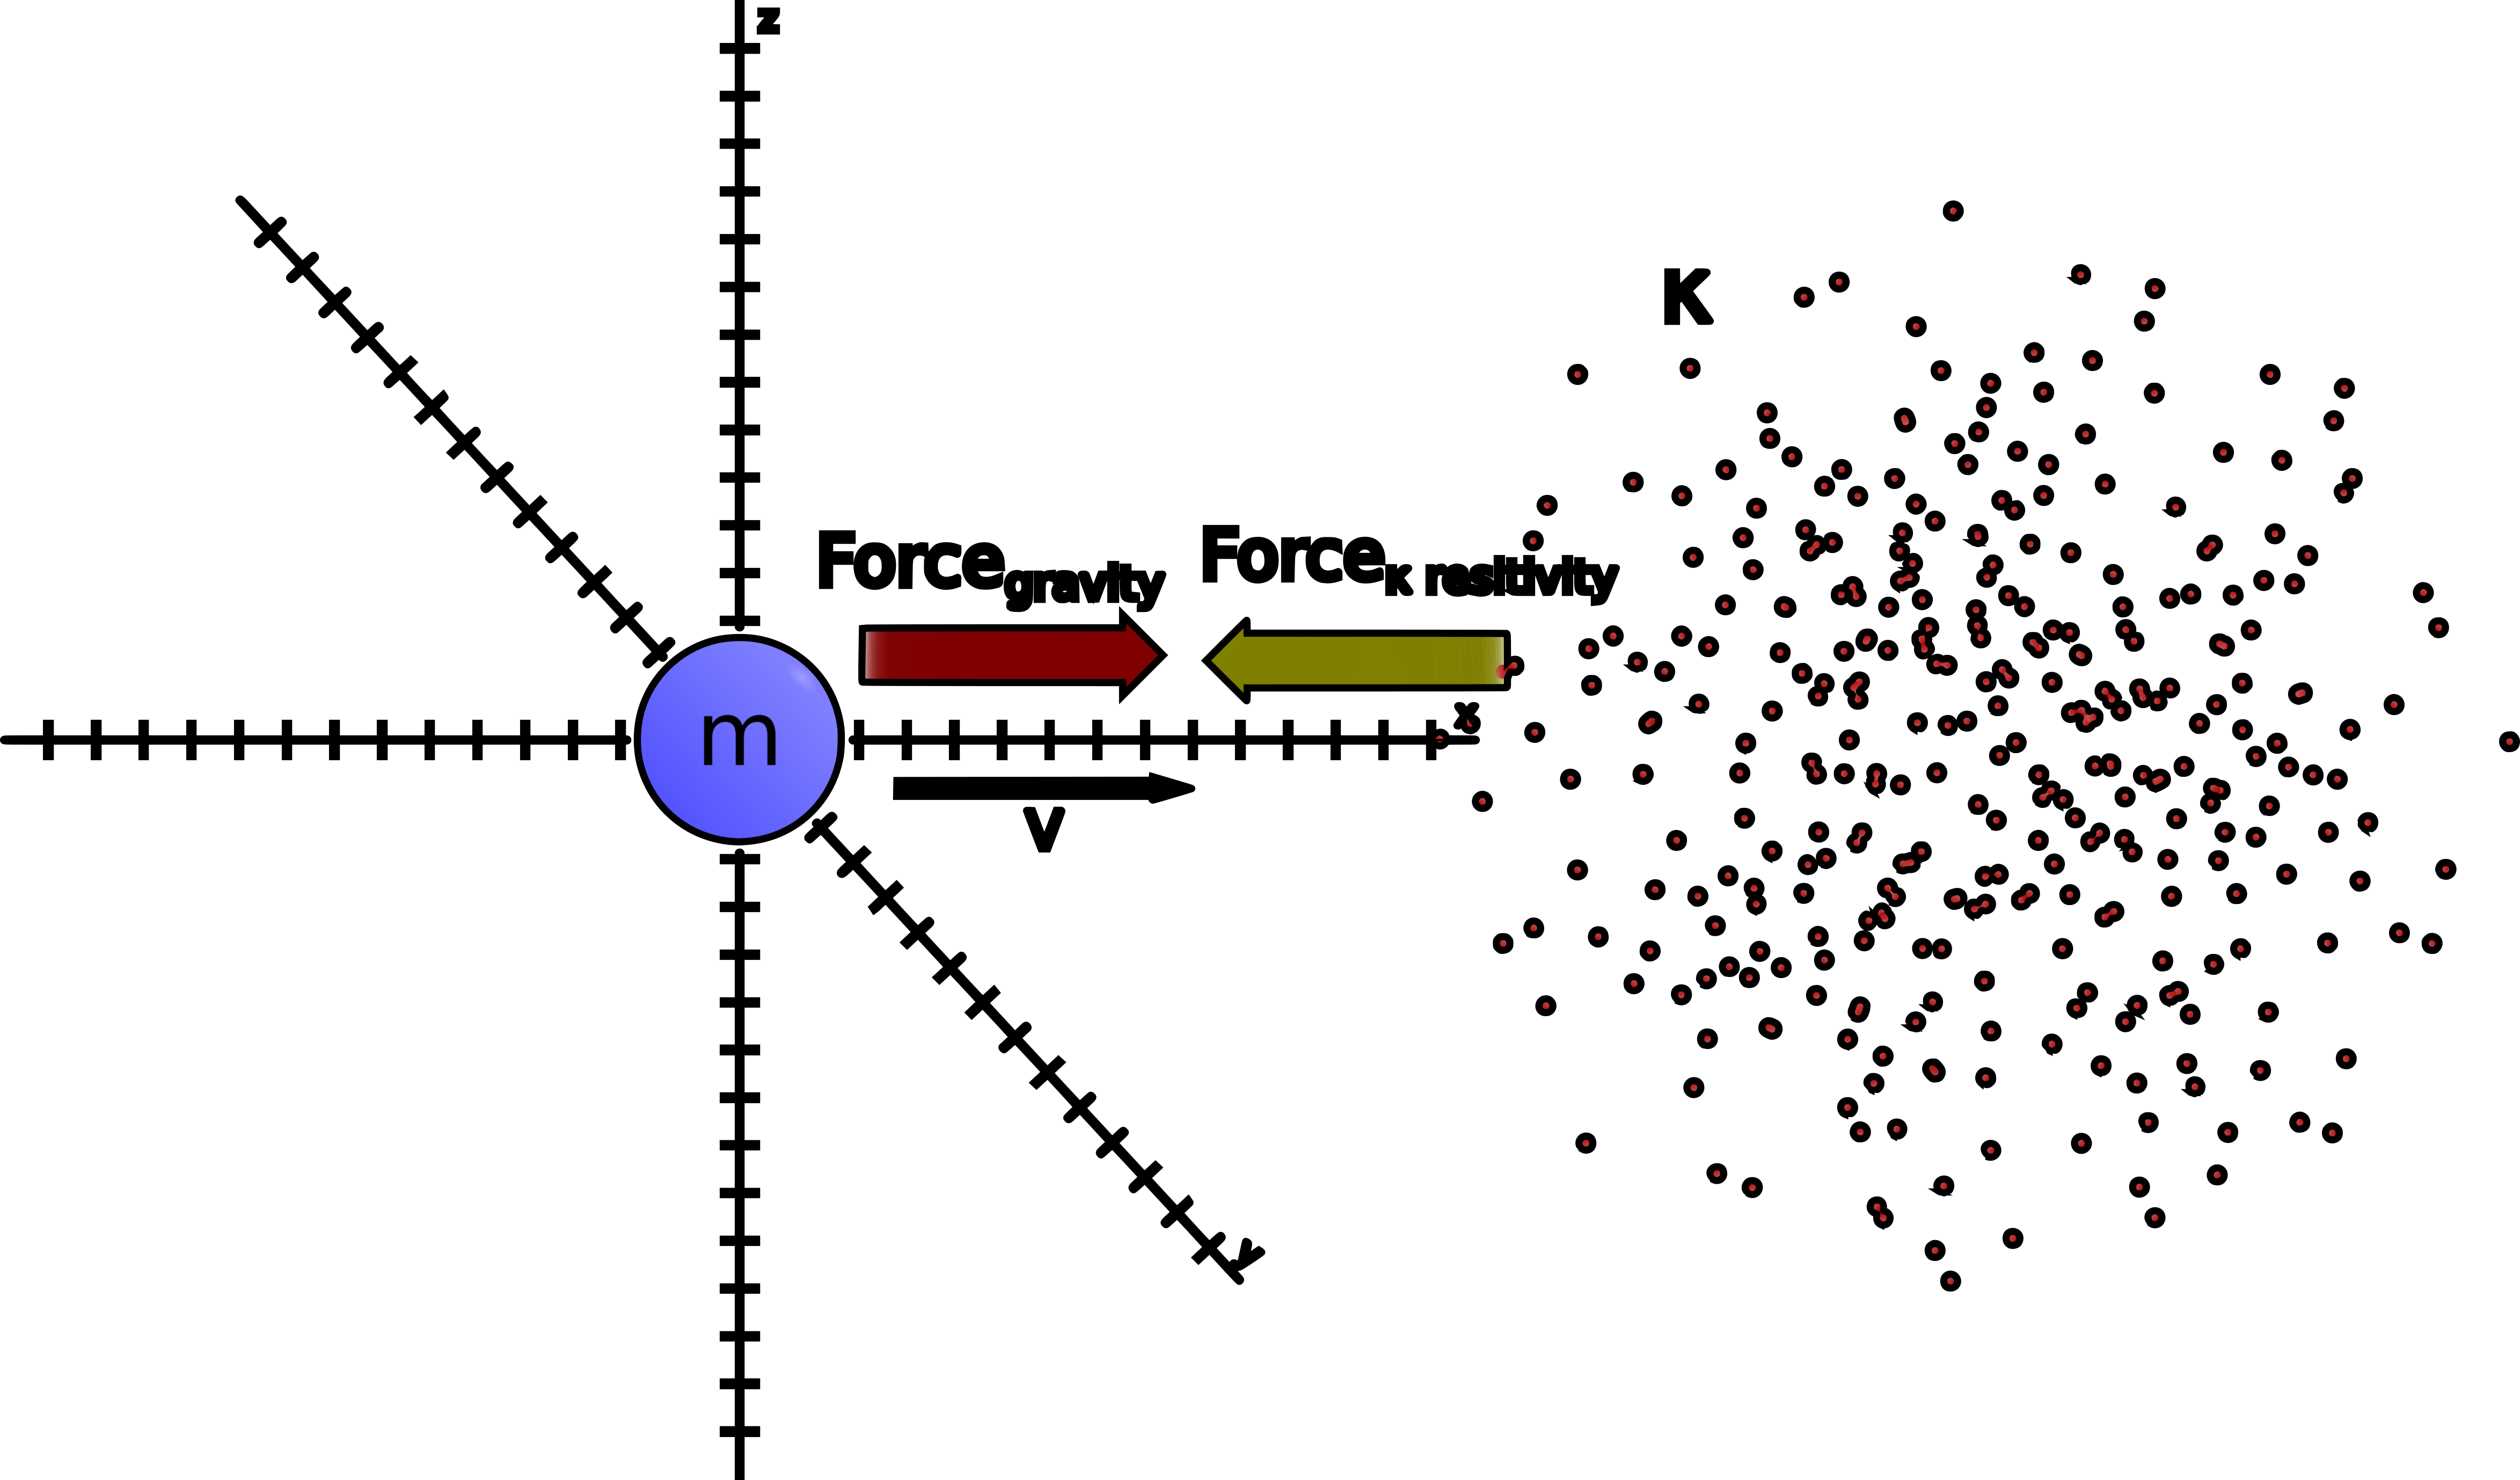
\includegraphics[scale=1]{coordinates}}
\centerline{\caption{Figure 3: Choice of coordinates.}}\\
\subsection{Model of $F_{\text{Resistance of }\kappa} \propto v^{n}$ where $n = 1$}
By definition, if $K$'s resistive force proportional to the velocity then there exists a constant $k$ such that $k \cdot v = F_{\text{Resistance of }\kappa}$. Therefore summing the forces yields:\\

\begin{equation}
\sum \text{Forces} = \text{Force}_{gravity} -  \text{Force}_{\kappa \text{ resistance}}= 0
\end{equation}

We know from Newtons second law that:

\begin{equation}
F = m \cdot \color{blue}a	\color{black}
\end{equation}

And acceleration is:

\begin{equation}
\color{blue}a\color{black} = \color{red}\dfrac{dv}{dt}\color{black}
\end{equation}

Therefore, we can rewrite (1) as:

\begin{equation}
\sum \text{Forces} = \text{Force}_{gravity} -  \text{Force}_{\kappa \text{ resistance}}= m \cdot g - k \cdot v = 0
\end{equation}
 
Finally assuming that the object has not yet reached terminal velocity implies that it is under acceleration. So (4) becomes:

\begin{equation}
\begin{align}
			m \cdot \color{blue}a\color{black} &= m \cdot g - k \cdot v\\
m\cdot \color{red}\tfrac{dv}{dt}\color{black} &= m \cdot g - k \cdot v
\end{align}
\end{equation}

This is a separable ordinary differential equation which is solved in Appendix A:

\begin{equation}
\begin{align}
					m\cdot\color{red}\tfrac{dv}{dt}\color{black} &= m \cdot g - k \cdot v\\				
\int\dfrac{m}{m \cdot g - k \cdot v}\cdot \color{green}dv\color{black} &= \int \color{green}dt\color{black}\\
\end{align}
\end{equation}

The solution is:

\begin{equation}
v = \dfrac{m \cdot g}{k} + \dfrac{v_{0}\cdot \textit{e}^{-\tfrac{k \cdot t}{m}}}{m \cdot g}
\end{equation}

The terminal velocity is then:

\begin{equation}
\begin{align}
\lim_{t \to \infty} v &= \dfrac{m \cdot g}{k} + \dfrac{v_{0}\cdot \textit{e}^{-\tfrac{k \cdot t}{m}}}{m \cdot g}\\
					v &\to \dfrac{m \cdot g}{k}
\end{align}
\end{equation}
It is interesting to note that the initial velocity is irrelevant to the terminal velocity. Also the mass is a factor in the terminal velocity. So in the presence of an atmosphere objects of different masses do not fall at the same speed. Only in a vacuum would object of different masses fall at the same speed. A substantial flaw in this model is that $k$ must be determined experimentally.\\

\subsection{Model of $F_{\text{Resistance of }\kappa} \propto v^{n}$ where $n = 2$}

Recalling equations (1),(2), and (3) from section 2.1 a model for the case where $n = 2$ can be constructed in a similar manner as the $n = 1$ case. The equation is worked out fully in Appendix B.

\begin{equation}
\begin{align}
						m \cdot \color{blue}a\color{black} &= m \cdot g - k \cdot v^{2}\\
m\cdot \color{red}\tfrac{dv}{dt}\color{black} &= m \cdot g - k \cdot v^{2}\\
\int\dfrac{m}{m \cdot g - k \cdot v^{2}}\cdot \color{green}dv\color{black} &= \int \color{green}dt\color{black}\\
\end{align}
\end{equation}
The solution is:
\begin{equation}
v = \dfrac{\sqrt{m \cdot g}}{\sqrt{k}}\cdot \left(\dfrac{-1 - c \cdot\textit{e}^{\tfrac{2\cdot g \cdot\sqrt{k}}{\sqrt{m \cdot g}}\cdot t}}{1 - c \cdot\textit{e}^{\tfrac{2\cdot g \cdot\sqrt{k}}{\sqrt{m \cdot g}}\cdot t}}\right)
\end{equation}

By taking the limit as $t \to \infty$ the terminal velocity is shown to be:

\begin{equation}
\begin{align}
\lim_{t \to \infty} v &= \dfrac{\sqrt{m \cdot g}}{\sqrt{k}}\cdot \left(\dfrac{-1 - c \cdot\textit{e}^{\tfrac{2\cdot g \cdot\sqrt{k}}{\sqrt{m \cdot g}}\cdot t}}{1 - c \cdot\textit{e}^{\tfrac{2\cdot g \cdot\sqrt{k}}{\sqrt{m \cdot g}}\cdot t}}\right)\\
v &\to \dfrac{\sqrt{m \cdot g}}{\sqrt{k}}
\end{align}
\end{equation}
A table comparing the differences in these two models is given in Appendix D. Without some predetermined value of $k$ neither of these models would help to determine what size parachute we need for a given mass m. Without experimental evidence it is impossible to know that an umbrella would not work to save your life if you jumped off of a bridge. Another issue with these models is that they do not predict the terminal velocity changing with a change in density of $\kappa$. So a better model is needed.

\subsection{Model of $F_{\text{Resistance of }\kappa} \equiv p \cdot A$}
Pressure is the sum of all the collisions of particles for a given area. If a gas was confined to a cube then its pressure would be the sum of all the collisions from all the sides for a given time.\\

\begin{equation}
\begin{align}

\text{Pressure} &= \tfrac{\text{Collisions}}{\text{Area_{0}}\cdot t}} + \tfrac{\text{Collisions}}{\text{Area_{1}}\cdot t}} &+ \tfrac{\text{Collisions}}{\text{Area_{2}}\cdot t}} + \tfrac{\text{Collisions}}{\text{Area_{3}}\cdot t}} + \tfrac{\text{Collisions}}{\text{Area_{4}}\cdot t}} + \tfrac{\text{Collisions}}{\text{Area_{5}}\cdot t}}
\end{align}
\end{equation}

\centerline{\includegraphics[scale=.5]{pressure_low}}
\centerline{\caption{Figure 4: A gas in a cube.}}\\

Without changing the number of gas particles or the volume of the cube, we can increase the pressure by heating the gas because $P \cdot V = N \cdot R\cdot T$. By heating the gas we increase the velocity of the gas as it strikes the faces of the cube. From (3) a change in velocity is by definition acceleration and by (2), assuming the gas has mass, an acceleration of mass is force. Therefore pressure is related to force and area by:

\begin{equation}
p = \dfrac{F}{A}
\end{equation}

\centerline{\includegraphics[scale=.5]{pressure_high}}
\centerline{\caption{Figure 4: Heated gas in a cube.}}\\

For the sake of argument let's assume that our cube is now solid and inside of a gas. Suppose the gas is stationary and the cube is in motion, (12) is now simplified becuase we only need to consider one face,the striking face of the cube, and one velocity, the cube's.

\centerline{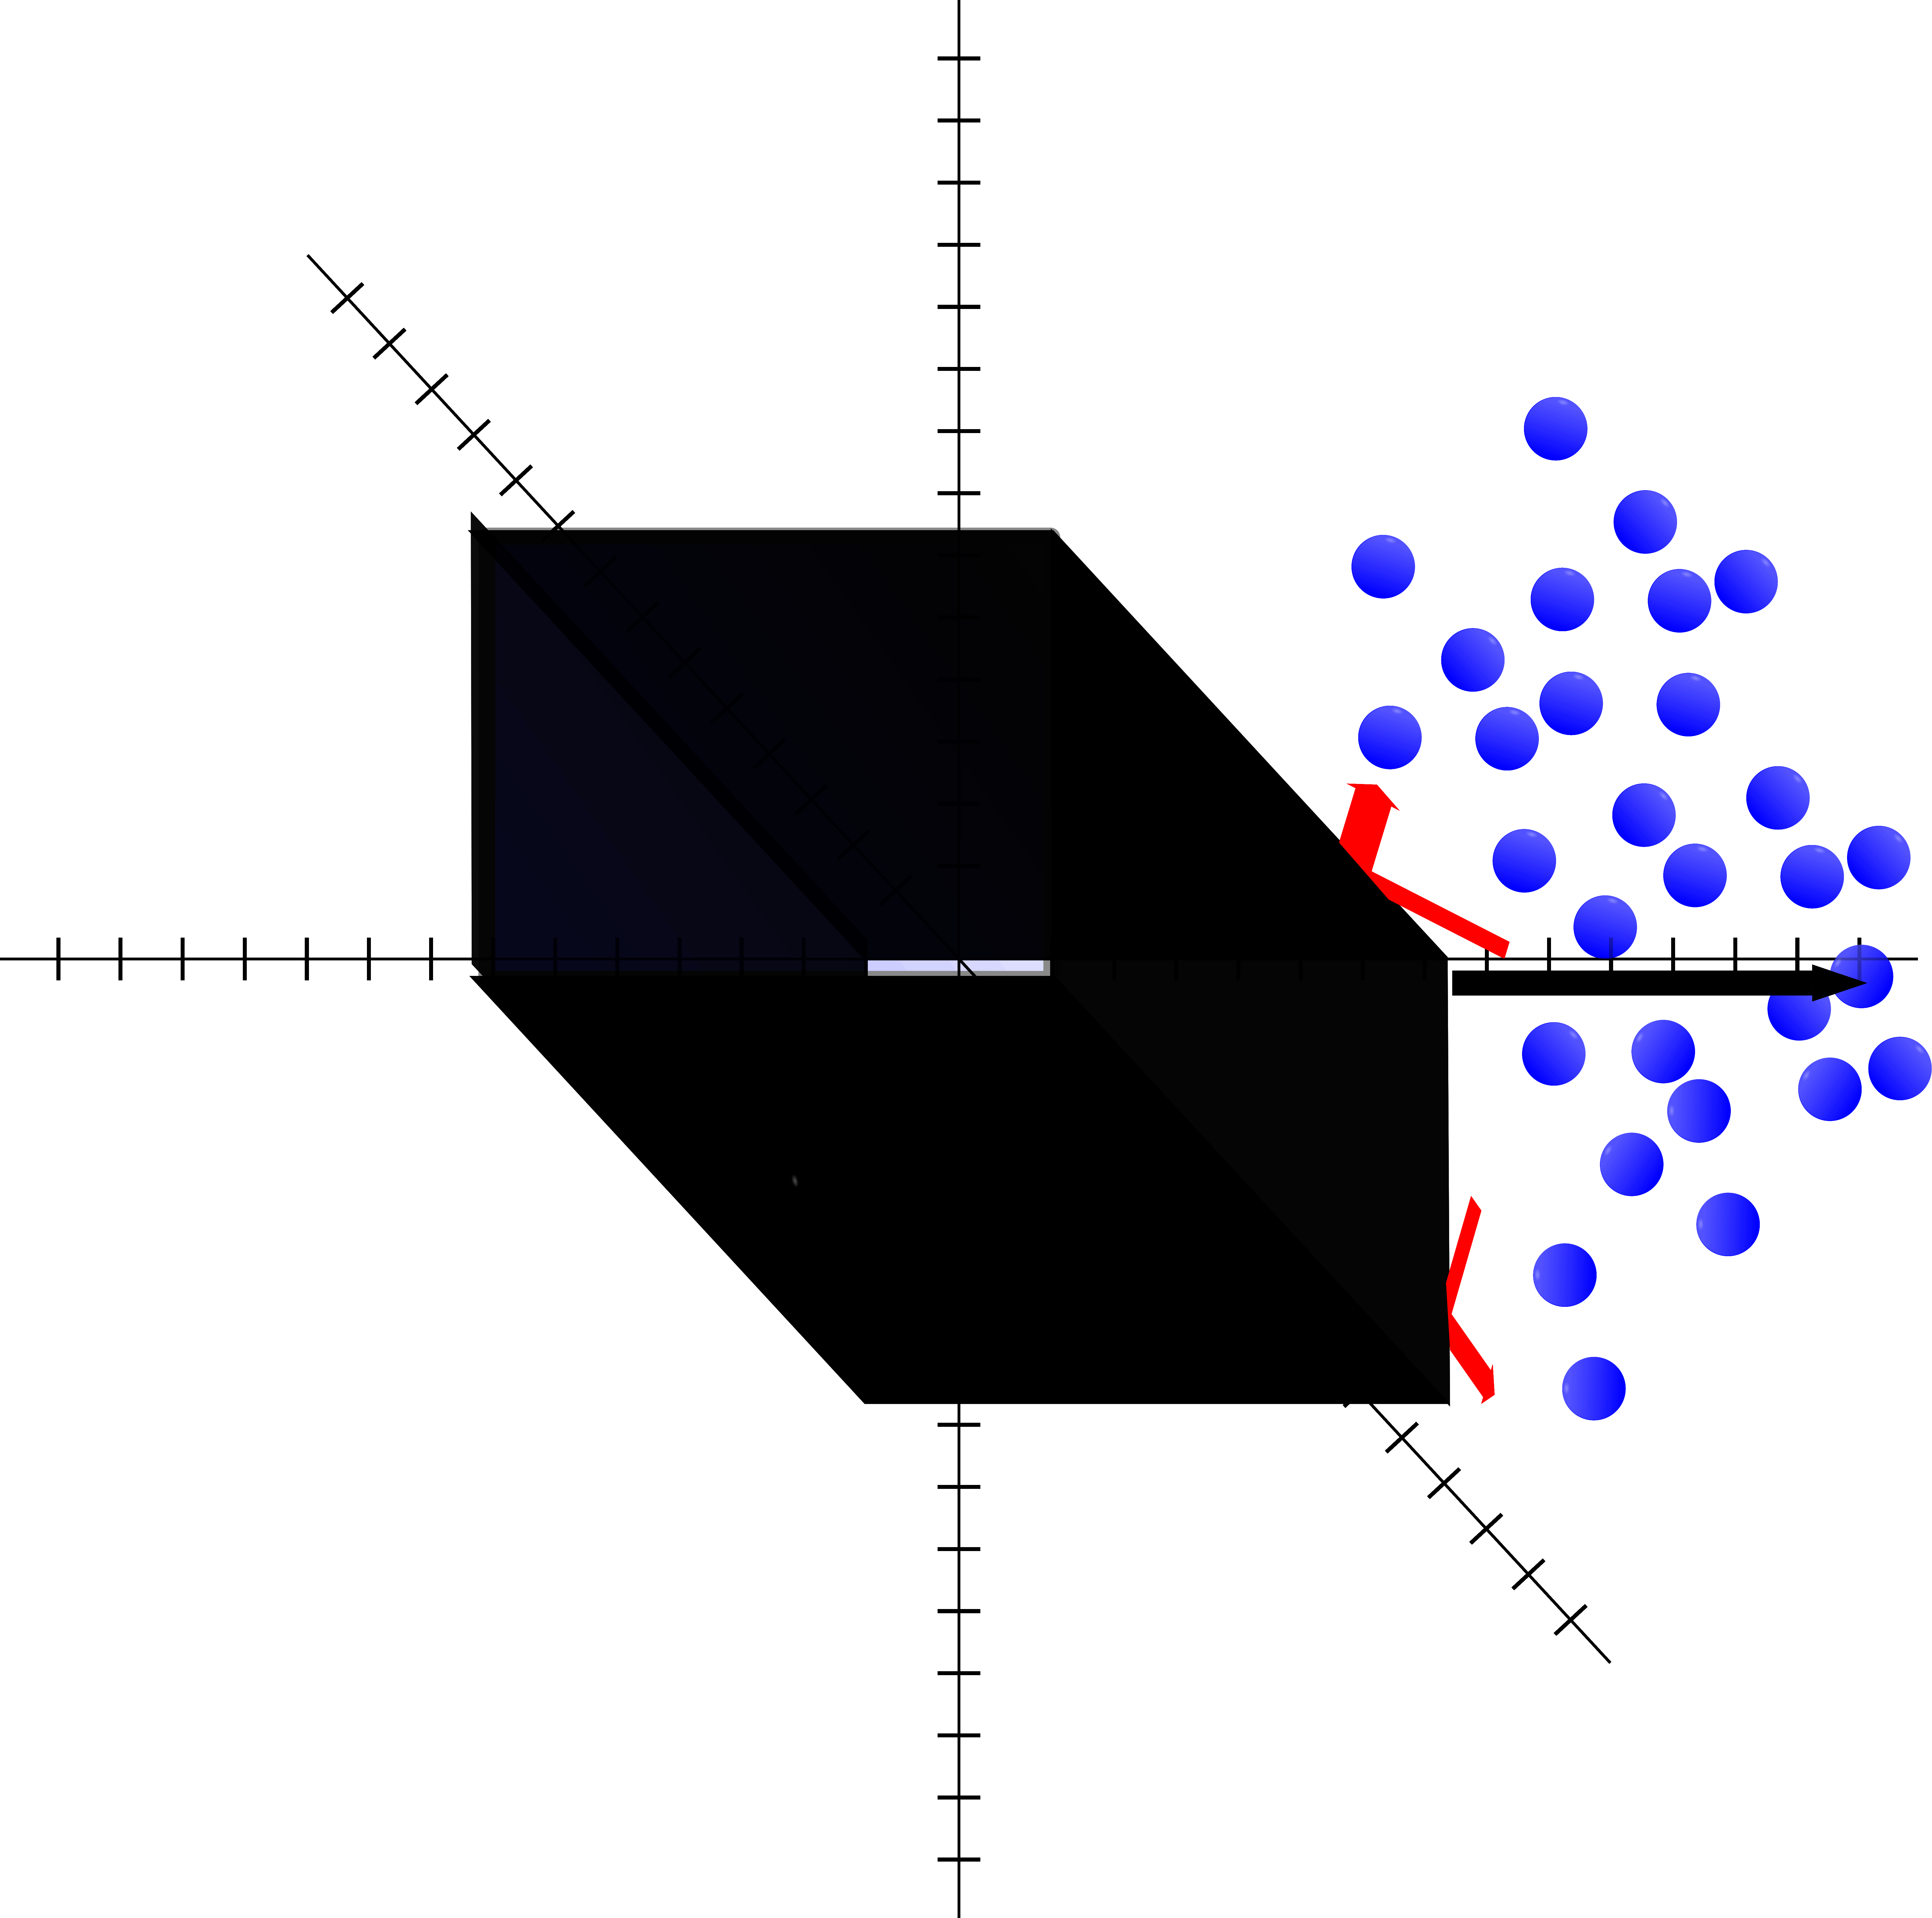
\includegraphics[scale=.5]{box}}
\centerline{\caption{Figure 5: Simplified version of (12) because only one face and one velocity to consider.}}\\

\end{document}